\section{Introduction}
% \lipsum[1-8]
\subsection{Problem Background}

Tennis has always been a sporting event that is watched by the masses and in the men's final of the 2023 Wimbledon Tennis Championships, 20 year old Spanish star Carlos Alcaraz defeated 36 year old Novak Djokovic in a tightly contested match. At the start of the match, Djokovic showed overwhelming power that seemed to signal an easy victory. But the match took a surprisingly volatile turn during the course of the match. In the end it was Carlos Alcaraz, who was not favored at the start of the match, who emerged victorious.

\subsection{Problem Restatement}

\begin{figure}[h]
    \centering
    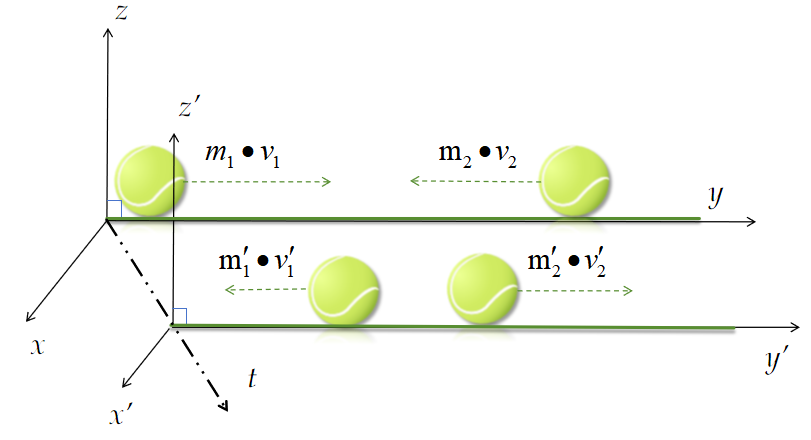
\includegraphics[width=0.7\textwidth]{figure/collision_of_tennis_balls(2).png}
     % \vspace{-0.3cm}
    \caption{The Momentum of Tennis}
    \label{fig:correlation_heatmap }
    % \vspace{-0.5cm}
\end{figure}
% 




Match swings are often linked to a player's momentum — the power or advantage gained. It's unclear how this momentum is generated or altered, prompting an examination of its role in matches and its predictive potential.

Given data from the 2023 Wimbledon Gentlemen's matches, including match ID, players' names, and elapsed time, we aim to use momentum observations to address the following problem:

\begin{itemize}[label=$\bullet$]
  \item Establish a model capable of analyzing player performance during a match, based on which the match process can be visualized and logically represented.
  \item Establish a traditional random probability model for comparison, assessing the role of momentum in the match.
  \item Analyze factors influencing turning points in a match from the following two perspectives:
    \begin{itemize}[label=\textbullet, itemsep=1ex]
       \item Develop a model for predicting match swings to analyze influencing factors.
       \item Provide players with recommendations to improve their chances of winning.
     \end{itemize}
 \item Evaluate the established predictive model for match swings based on the following two criteria:
    \begin{itemize}[label=\textbullet, itemsep=1ex]
       \item Analyze the accuracy of swing predictions, considering factors that may contribute to improving the model's accuracy when performance is subpar.
       \item Consider adding additional factors to enhance the model's generalizability.
    \end{itemize} 

\end{itemize}

\subsection{Our Work}
%%%%%%%%%%%%%%%%%%%%%%
%%% TODO
%%%%%%%%%%%%%%%%%%%%%%

\begin{figure}[h]
    \centering
    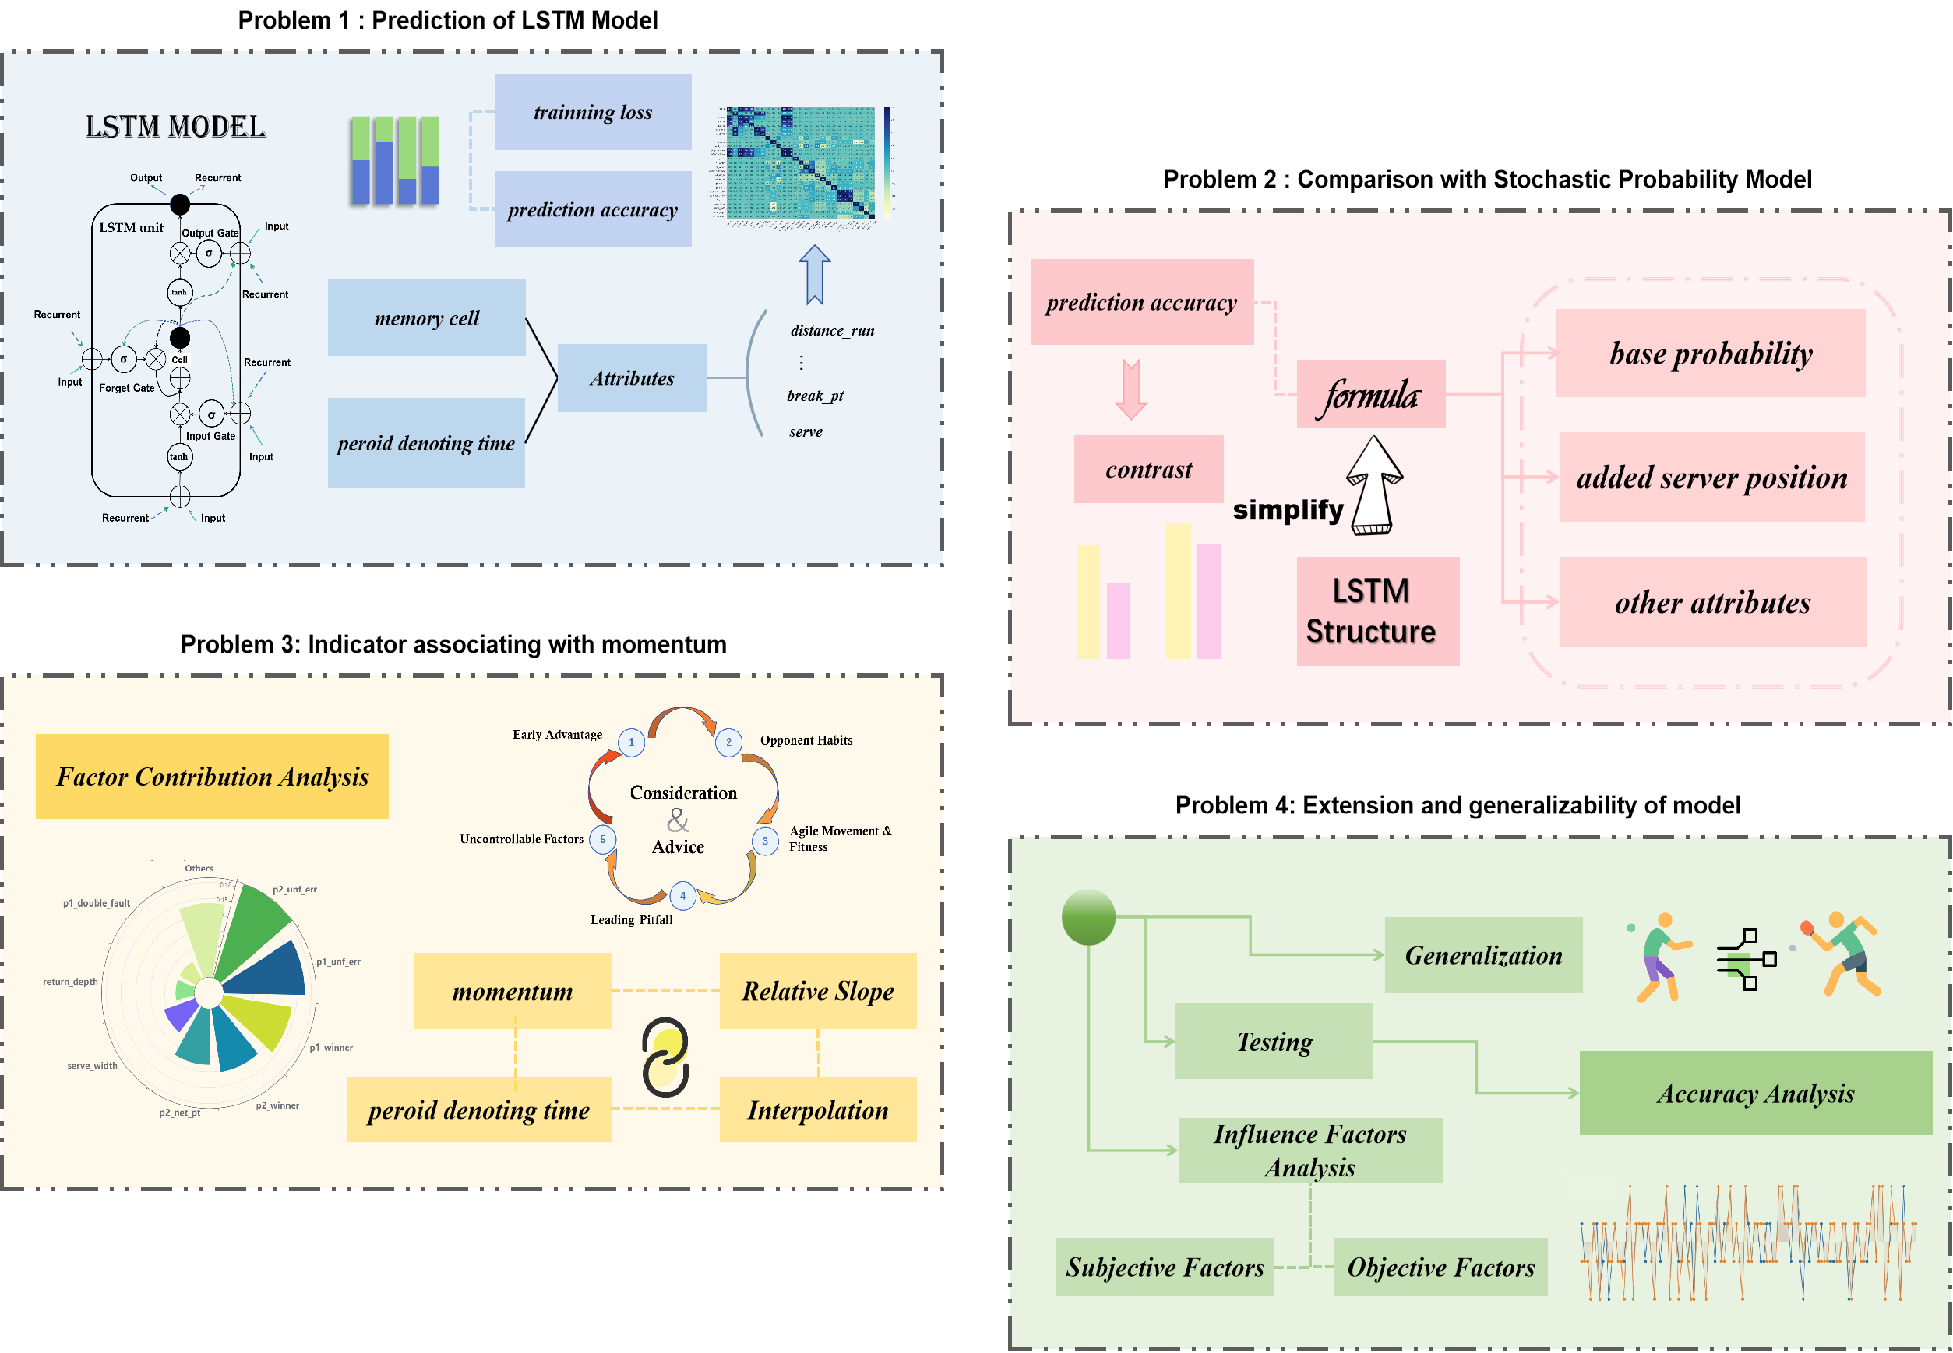
\includegraphics[width=1\textwidth]{figure/3.png}
     % \vspace{-0.3cm}
    \caption{Overall Architecture Diagram}
    % \vspace{-0.5cm}
\end{figure}

% 在问题一中,我们依据动量随时间的变化这个条件选取LSTM作为基础模型建模,重点观察动量的时间变化特点。首先我们对给定数据中字符串值的数据进行数字化,然后再归一化,去掉量纲。接下来我们分析了各种指标之间的相关性,选取其中独立性相对较强的部分,作为LSTM模型的输入,同时将数据集划分为训练集和测试集,经过大约六个小时的训练,得到准确率极高的模型输出。

In problem 1,\textbf{ we select LSTM as the foundational model based on the condition of momentum changing over time}, focusing on observing the temporal characteristics of momentum. Firstly, \textbf{we digitize the string values in the given data, followed by normalization to remove scale differences. }Subsequently, we analyze the correlations among various indicators, selecting those with relatively strong independence as inputs for the MM-LSTM model. Additionally, we divide the dataset into training and testing sets. After about 6 hours training, we obtain a highly accurate model output.

% 问题二要求我们以随机概率模型进行预测计算,与第一问的模型进行对比。我们首先对LSTM模型的原理进行剖析,整理得到其计算的核心公式,再通过对公式的抽象简化,得到可计算的简化的传统概率模型,同时降低了计算的复杂度。在这个模型中我们继续减少影响因素的个数,尽管计算得到的概率较低,但是相对于估计的真实的概率偏差不太大。同样这也说明了动量对于比赛得分的重要性。

In terms of problem 2, we conduct predictive calculations \textbf{using a random probability model and compare it with the model in problem 1}. We begin by analyzing the principles of the LSTM model,\textbf{ extracting its core formulas, and then abstracting and simplifying these formulas to obtain a computationally simplified traditional probability model}. This approach reduces computational complexity while maintaining calculability. In this model, we further reduce the number of influencing factors. Despite obtaining lower probabilities, the deviation from the estimated true probabilities is relatively small. This also underscores the significance of momentum in determining match scores.

% 经过我们对问题三题干的分析,相较于选择其他复杂因素的预测思路,我们剖析潜藏在历史胜负洪流中微不可查的动量变化。经过精密的数学推导,最终我们得到斜率相对差与动量之间的关系,发现了动量的变化原因和预报条件。同时我们也在训练中同步进行梯度重要性分析,得到影响准确性的主要因素。基于这些和对数据的分析计算,我们对运动员提出了基于“动量”的建议。我们对比赛开始以及过程中的动量波动分析,又对物理因素进行计算,最终总结提出五条有效建议。

After our analysis of the problem 3 prompt, in contrast to choosing prediction approaches involving other complex factors,\textbf{ we dissect the subtle momentum changes hidden within the historical win-loss dynamics}. Through precise mathematical derivations, we ultimately \textbf{establish the relationship between the relatively differential slope and momentum, uncovering the reasons for momentum changes and forecasting conditions.} Simultaneously, we conduct gradient importance analysis during training to identify the primary factors influencing accuracy. Based on these analyses and computations, we propose recommendations for athletes based on momentum. We compare momentum swings during the start and throughout the match, perform calculations related to physical factors, and ultimately summarize and \textbf{present five effective suggestions}.

% 在解决问题4的时候,我们首先使用LSTM模型预测的结果来绘制动量波动图像,并且计算出超过90%的准确性,证明了模型的优秀。同时我们在原本的因素的基础上拓展,查找文献资料,分别从主观和客观两个方面对于其他可能出现的因素进行分析。我们还在网络上搜集了乒乓球比赛的数据,将建立的LSTM模型应用到对乒乓球比赛数据的预测分析上,也得到了较好的效果。

In addressing problem 4, we initially employ the results predicted by the MM-LSTM model to generate momentum swings images, \textbf{achieving an accuracy exceeding 90\% and confirming the model's excellence}. Simultaneously, we expand on the original factors, conduct literature reviews, and \textbf{analyze other potential factors} from both subjective and objective perspectives. Additionally, we collect table tennis match data from online sources and apply the established MM-LSTM model to predict and analyze table tennis match data,\textbf{ yielding favorable outcomes}.

